\section{Automatic Detection of XML Signature Wrapping Attacks}
\label{sec:automatic_detection_of_xml_signature_wrapping_attacks}

XML Signature Wrapping (XSW) is a Web Service specific attack allows to modify signed
XML messages. 
It was firstly published in 2005 by McIntosh and Austel~\cite{xsw}. 
The basic idea of this attack is to trick out the reference mechanism which detects the signed parts
of an XML message and thus let it use a different message part than the application
logic uses.

The impact of this attack can be seen in~\cite{amazon} where the authors uses an XSW attack to
attack the Amazon EC21 and Eucalyptus2 SOAP interfaces. They only need to eavesdrop
a single SOAP message and afterwards, they are able to start, stop and download the
victims cloud instance.

In 2012, the authors applied the attack technique to Single Sign-On scenarios and successfully attacked 11 out of 14 SAML frameworks, including Shiboleth and IBM DataPower~\cite{samlattacking}.

The WS-Attacker XSW Plugin and Library is mainly based on a Master Thesis by Christian Mainka\footnote{\url{http://nds.rub.de/media/nds/arbeiten/2012/07/24/ws-attacker-ma.pdf}}.

\subsection{Short Technical Attack Description}
\label{sec:short_technical_attack_description}

The most frequently used scenario for XML Signature is to refer the signed parts of an XML message by an ID attribute. 
This method is easy to understand for humans and simple to implement for developers. 
However, it has the big disadvantage that the signature itself only protects the content of the signed elements but not its location within the document. 
Thus, the signed element can be moved to another location -- vertically and horizontally in the Document structure -- without invalidating the signature. 

Figure~\ref{fig:xsw_id} gives an example for constructing an XSW message which still bypasses the signature verification process but changes the payload used by the application logic.

\begin{figure}[ht]
    \begin{center}
        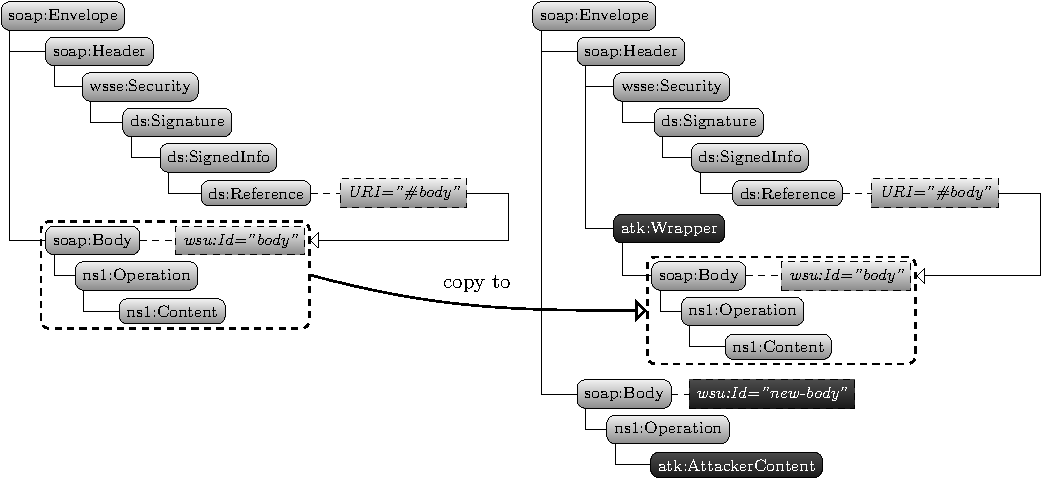
\includegraphics[width=\linewidth]{img/xsw_id}
    \end{center}
    \caption{Creating an XSW message for an ID referencing based XML Signature. 
The original signed message is shown on the left side.
The XSW message on the right side is constructed by copying the signed element to a \texttt{Wrapper} element and modifying the signed content to the attackers' needs.}
    \label{fig:xsw_id}
\end{figure}

The original message has a signed \texttt{Body} element which is referenced by the ID attribute \texttt{\#body}.
The attack message on the right has a new \texttt{Wrapper} element placed as a child of the \texttt{Header} element.
Its child is a copy of the original signed \texttt{Body} element.
Note that the ID attribute still has the value \texttt{\#body}.
The original \texttt{Content} element is replaced by a new \texttt{AttackerContent} element and the ID attribute of its ancestor \texttt{Body} element is changed to \texttt{new-body}, so that the signature verification logic will not use it.
There might also be other attack scenarios in which the attribute value remains the same as in the \texttt{Wrapper} element or it removed completely.
The success of this attack depends on the implemented application- and verification logic.

The main problem why this attack works is that the signature verification- and the application logic use different methods for detecting their elements.
The signature verification logic looks for an element which has the attribute \texttt{wsu:Id="body"} and uses it to compute the digest value.
The application logic, in contrast, does not care about the attribute \texttt{wsu:Id="body"} -- it just uses the first child element of the \texttt{Body} element in the SOAP message.
Obviously, these referencing methods are not equivalent, as the example attack message shows.

This is just the very basic example of one possible XSW techniques. More complicated attack variants can be found in~\cite{Liao2011},~\cite{2011:07:xmlSigConSAPSE} and the Master Thesis mentioned before.

\subsection{Using the XSW Plugin}
\label{sec:using_the_xsw_plugin}

This section will explain how to use the XSW plugin by an example attack on Apache Axis2 which uses the Rampart Security Module. 
For attacking the server, it is started with the policy example 02 distributed with Rampart. 

The first steps are similar to the common usage of WS-Attacker. 
You need to load the WSDL and choose the operation to attack. 
Afterwards you need a signed SOAP message to continue. 
Creating/Getting such messages can be a real challenge. 
One example to create such a message is to use SoapUI\footnote{\url{http://www.soapui.org/}}. 
However, this tool is only capable for creating ID based XML Signatures. 
Another example is using Wireshark4 and eavesdrop a message created by some client. 
For this scenario, the message created by the Rampart example client is eavesdropped. 

Next is to configure the plugin. Figure~\ref{fig:xsw_plugin_config} shows the configuration window.

\begin{figure}[ht]
    \begin{center}
        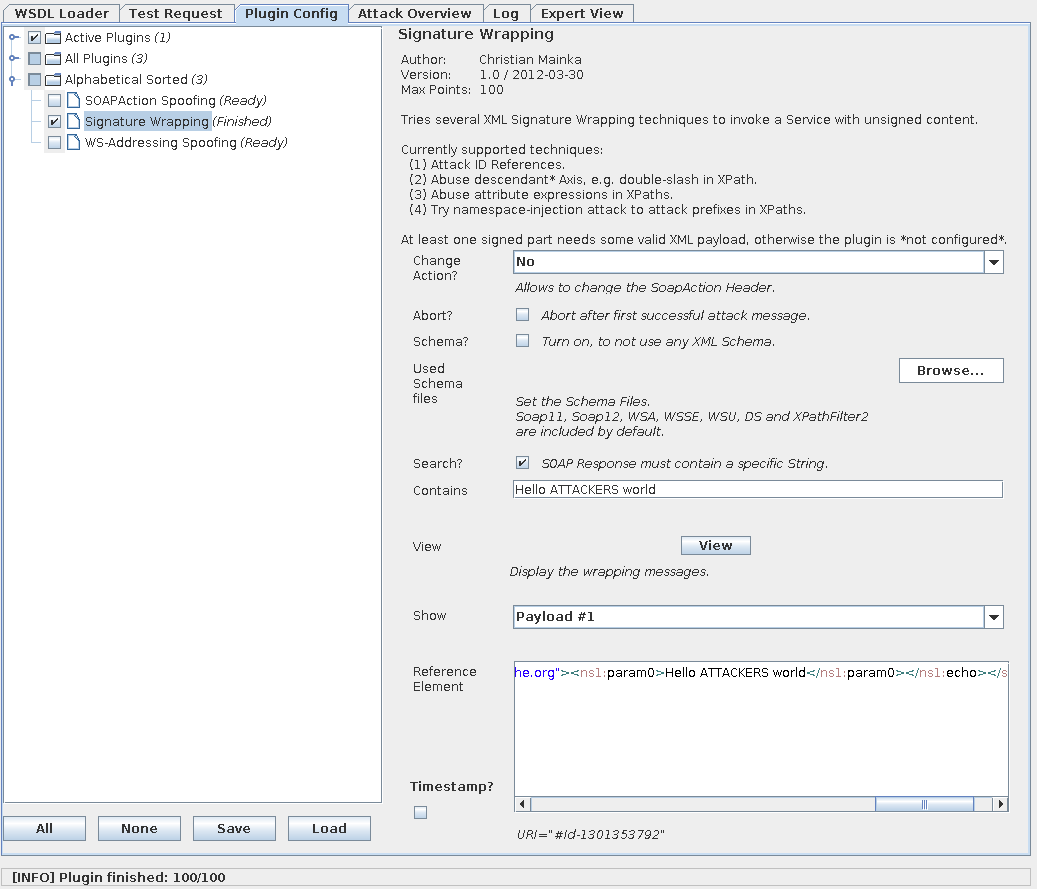
\includegraphics[width=0.9\linewidth]{img/xsw_attacking_axis_with_policy_config}
    \end{center}
    \caption{Configuration of the XSW plugin within the WS-Attacker framework.}
    \label{fig:xsw_plugin_config}
\end{figure}

\begin{itemize}
    \item It is possible to \textbf{change} the \textbf{SOAPAction} parameter. This can be useful if the attacker wants to invoke a different operation to the one he chose after loading the WSDL.
    \item If the \textbf{abort} checkbox is on, the attack will stop after the first successful attack. Otherwise, it will go on with further XSW messages. This can be usefull to detect more than one attack message.
    \item The \textbf{Schema Validation} can be optionally turned off. This might be useful if the server does not care on any XML Schema. However, the attack will be much slower as more XSW attack messages can be used.
    \item An optional \textbf{Search String} can be specified. This means, that each response, which is not a SOAP Fault, will be searched for this string. The attack is then only successful if the string is contained. This is useful to detect if the correct payload is used (in some cases, the original payload can be executed instead of the new one).
    \item A \textbf{view button} can be used to create and view all XSW messages without sending them to the server. If the WS-Attacker user knows the ID of the successful message (shown in log), he can use this button to re-create the message.
    \item The \textbf{dropdown} box must be used to set the payload. Note that the plugin is \textbf{not configured} if there is no payload set by the user.
\end{itemize}

After configuring the plugin, the attacks can be started as usual. An example result
window can be seen in Figure~\ref{fig:xsw_plugin_result}.

\begin{figure}[ht]
    \begin{center}
        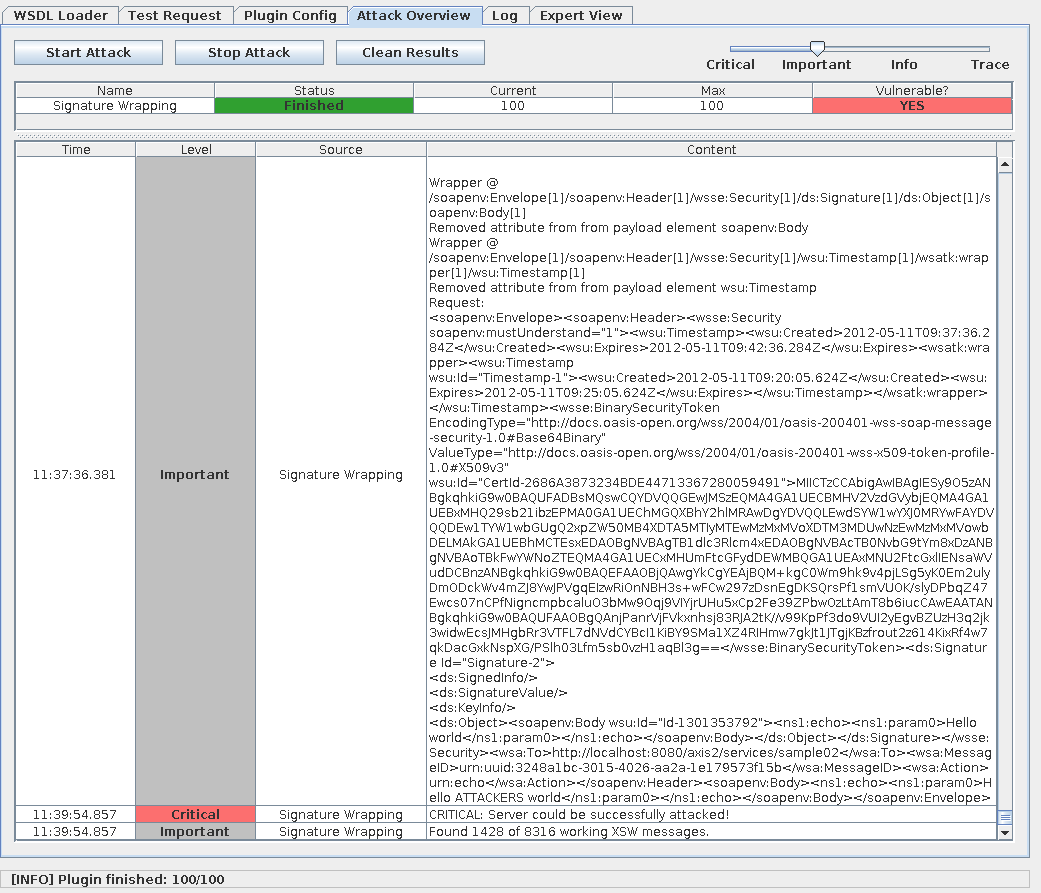
\includegraphics[width=0.9\linewidth]{img/xsw_attacking_axis_with_policy_result}
    \end{center}
    \caption{Results of the XSW plugin.}
    \label{fig:xsw_plugin_result}
\end{figure}
